% \usepackage{float}
% \usepackage{mathtools}
% \usepackage{amsthm}
% \theoremstyle{definition}
% \newtheorem{example}{Example}[section]
% \newtheorem{problem}{Problem}[section]
\begin{activity}{Gradients Activity}

\epigraph{ ``I will never listen to ocean waves or view a beautiful sunset in quite the same way again. That is perhaps the greatest gift one can gain by delving into calculus: It is a whole new way of looking at the world, accessible only through the realm of mathematics.''}
{{\normalfont ---\ Jennifer Ouellette}, The Calculus Diaries: How Math Can Help You Lose Weight, Win in Vegas, and Survive a Zombie Apocalypse}

\section{Introduction}
As we study geophysical theory it will become clear that in order to unlock the secrets of the physical world, we must understand the changing nature of fields.  If the fields were constant the world would be very boring indeed, for it would not contain any variations in physical properties that we could remotely sense.  Variations in physical fields help us better understand the state (temperature, pressure, and composition), structure, and/or the evolution of our wonderous planet.  One of the simplest ways to explore a field is to examine the rate of change of the field, or gradient, which is really a fancy way of saying slope.

In this workshop you will explore conceptually the physical meaning of a gradient using intuitive examples from elevation.  We will be able to see how the gradient depends upon the direction we consider and how a derivative can be calculated simply for a complex geometry, and how the gradient of a scalar field such as elevation results in a vector field requiring both magnitude and direction in order to describe the gradient.

We will start the exercise by building a conceptual understanding of the gradient before creating a more complete mathematical description.

\section{Mount Shasta Example}
\begin{figure}[htb]
    \centering
    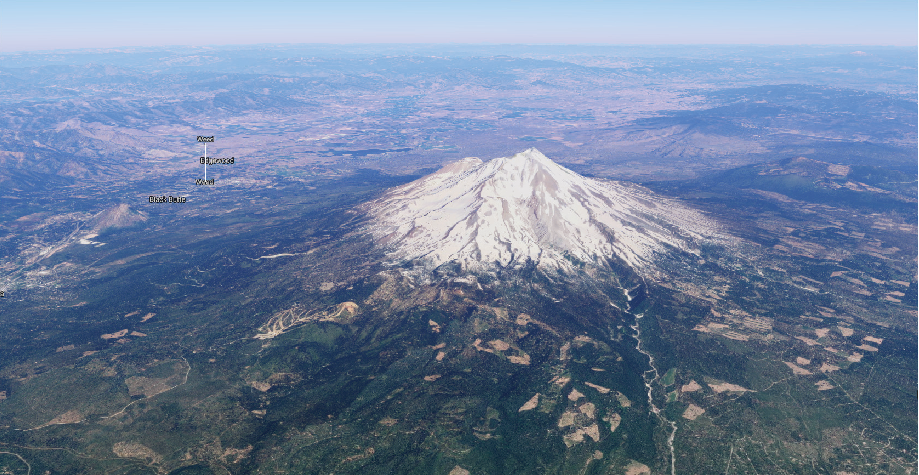
\includegraphics[width=0.75\textwidth]{activities/figures/mount_shasta.eps}
    \caption{Mount Shasta, California (image from Google Earth).}
    \label{fig:ms}
\end{figure}
Elevation is a good place to start to think about gradients because we all intuitively know what a slope means in this context.  As far as topography goes, Mount Shasta is pretty simple.  It is a stratovolcano at the southernmost end of the associated with the Cascade Volcanic Arc, and looks like a textbook example of a volcano in that it is fairly symmetric radially and sits in the middle of a vast flat plain.
\FloatBarrier

\begin{questions}
    \question{Shasta gradient}
    \begin{figure}[htb]
        \centering
        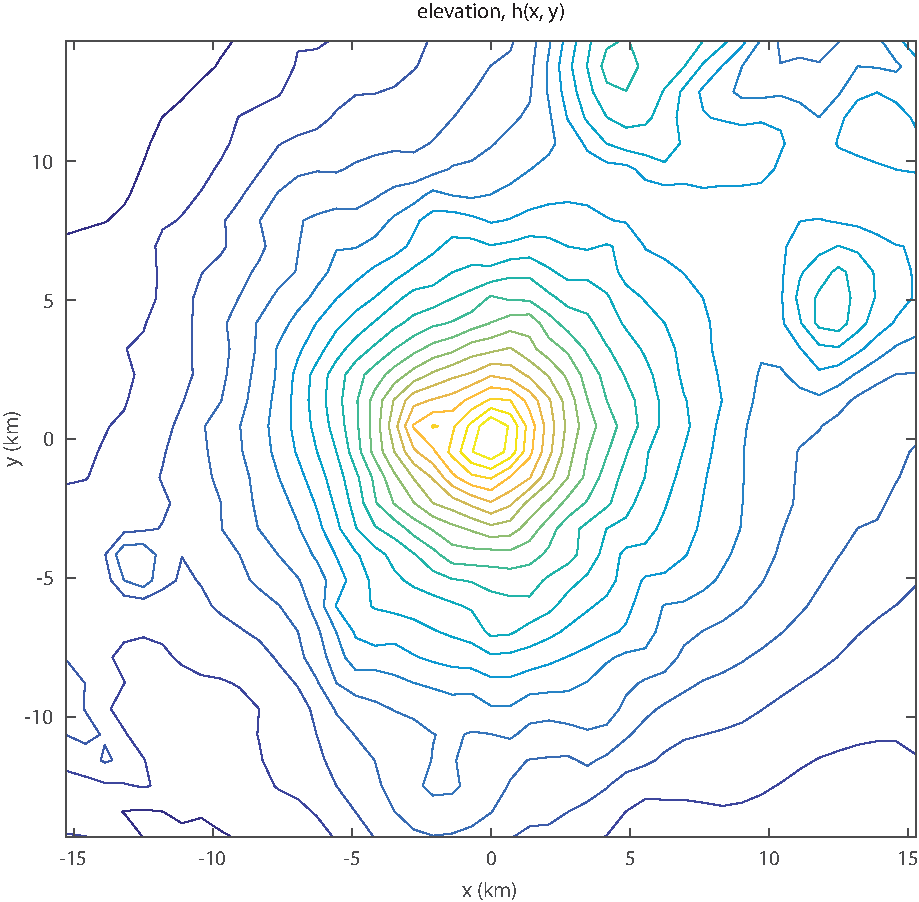
\includegraphics[width=0.6\textwidth]{activities/figures/mt_shasta_elevation.eps}
        \caption{Topographic map of Mount Shasta.}
        \label{fig:ms_elev}
    \end{figure}

    \begin{parts}
        \part Over the topographic contours on Figure~\ref{fig:ms_elev}, draw a series of arrows pointing up slope representing the opposite direction water might flow.  Make the arrows longer when the slope is steeper and make the arrows shorter when the slope is gentler.

        \part How did you decide to draw the direction of the arrows?
        \answerbox[2cm]

        \part How did you decide to draw the length of the arrows?
        \answerbox[2cm]

        \part Why does it require two quantities, length and direction, to describe the gradient?
        \answerbox[3cm]
    \end{parts}
\end{questions}
\FloatBarrier

% Compare the arrows you drew to the ones below shown below.  How well did you do?  If you find significant differences between your result and the true result, why is there a difference?  You'll probably notice that there are some features that this model shows that you didn't see (your topographic map isn't as high resolution as the dataset it is based on).

% \clearpage
% \begin{figure}[htb]
%     \centering
%     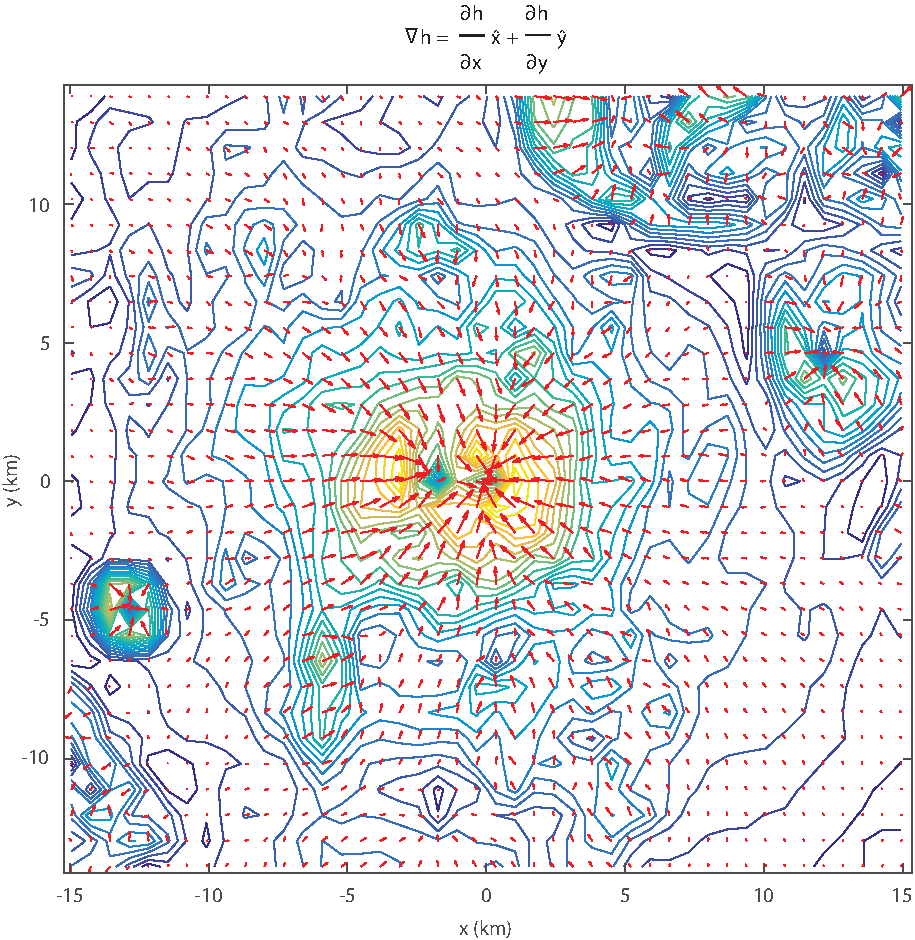
\includegraphics[width=0.75\textwidth]{activities/figures/mt_shasta_gradient.eps}
%     \caption{Gradient magnitudes (contours) and directions (arrows) of Mount
%     Shasta.}
%     \label{fig:ms_dxdy}
% \end{figure}

\section{The mathematics of gradients: the slopes of Mt. Shasta}

Consider hiking a profile line over the peak of Mt. Shasta (Figure~\ref{fig:profile}, top panel).  You will start by walking up the slope of Mt.  Shasta.  The slope starts gently going up in elevation (a positive slope in Figure~\ref{fig:profile}, bottom panel), which increases as you climb in elevation.  The slope increases and reaches a maximum near the peak, then the slope starts to decrease as elevation still increases.  Once you reach the snow-capped peak there is no change in slope (i.e., slope = 0).  Then you decide to pull out your sled and quickly decend the other side (negative slope).
\begin{figure}[htbp]
    \centering
    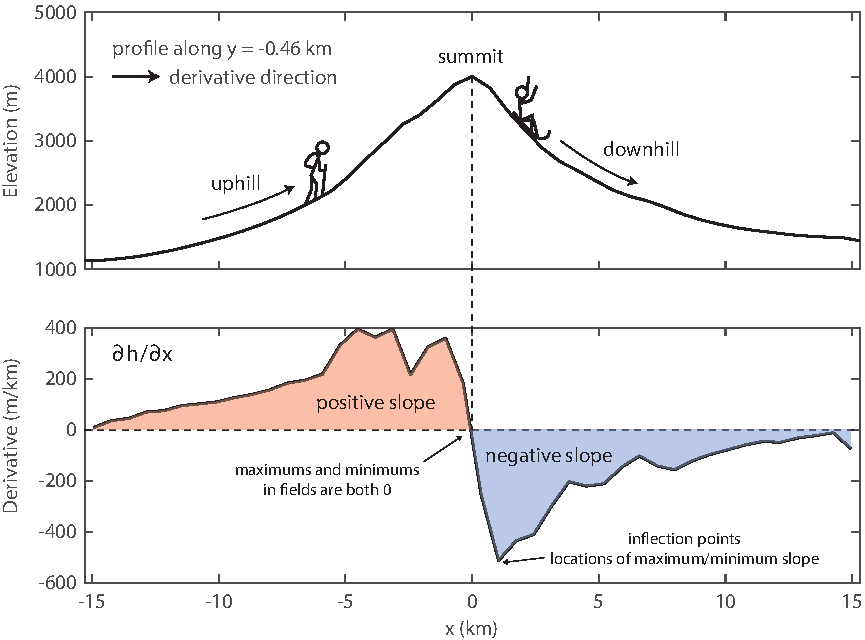
\includegraphics[width=0.75\textwidth]{activities/figures/mt_shasta_xprofile.eps}
    \caption{Elevation profile (top) and gradient along the elevation profile
    (bottom).}
    \label{fig:profile}
\end{figure}

What we want to do is be able to describe the changes in slope that you as a hiker feels mathematically.  Say every step you take is a similar distance laterally (the run) and the height you go up (or down, negative up) in elevation (the rise) allows us to express the slope as
\begin{equation}
    \text{slope} = \frac{\text{rise}}{\text{run}}.
\end{equation}
But the direction that you take matters.  Since we don't necessarily know the direction of the maximum slope we'll force the hiker to walk in just one direction, say west to east (+$x$) to start.  The size of the steps they take are $\Delta x$.  In this case, we can express the slope as
\begin{equation}
    \pdv{h}{x} \approx s_x = 
        \frac{h(x + \Delta x) - h(x)}{(x + \Delta{x}) - x} =
        \frac{h(x + \Delta x) - h(x)}{\Delta x}.
\end{equation}
At this point the way we solve this mathematically as opposed to a computer are different.  A computer will solve the problem much like above, taking the difference between the heights at $h(x + \Delta x)$ and $h(x)$ and dividing by the distance of each step ($\Delta x$).
\begin{framed}
    For our purposes generally during the course, we will take a more mathematical approach, taking the case where we want to know the slope at a continous series of point along the elevation profile.  In this case the distances between our steps approach zero and the slope we approximate the approaches a limit of the true slope at each point.  This is the definition of the derivative, and you can find an extended discussion as a tutorial online and in the math appendicies in the course notes.
\end{framed}

If instead, you were to hike from south to north (+$y$-direction) we we can write the slope as
\begin{equation}
    \pdv{h}{y} \approx s_y = 
        \frac{h(y + \Delta y) - h(y)}{(y + \Delta{y}) - y} =
        \frac{h(y + \Delta y) - h(y)}{\Delta y}.
\end{equation}

If you were to walk in a series of profiles in x or y, you could map out the slope with respect to that series of traverses.  You will notice that the slope you get is very different depending upon whether you walked in the x-direction or the y-direction
\footnote{Since Mt. Shasta is fairly radially symmetric, you will notice that the results are pretty similar if you rotate the one of the plots 90$^\circ$ with respect to the other.  This is a relatively special case as we can't generally do this, however, many of the problems we will solve in this course either change in one direction only or are symmetric in some way to make the problems simpler.}.  We can write the function of the slope, $s$ at each location $(x,y)$ as
\begin{equation}
    \vb{s}(x,y) = s_x \vu{x} + s_y \vu{y},
\end{equation}
where the $\vu{x}$ and $\vu{y}$ are a unit vectors in the $x$- and $y$-directions, respectively.  Note that the slope is a vector quantity, which means it has both a magnitude and a direction.  In calculus, we describe the gradient ($\grad$) of the elevation function, $h(x,y)$, by
\begin{equation}
    \grad{h} = \pdv{h}{x} \vu{x} + \pdv{h}{y} \vu{y} .
\end{equation}
Because the components are in different directions, we cannot simply add them to find the maximum slope.
% \begin{figure}[htb]
%     \centering
%     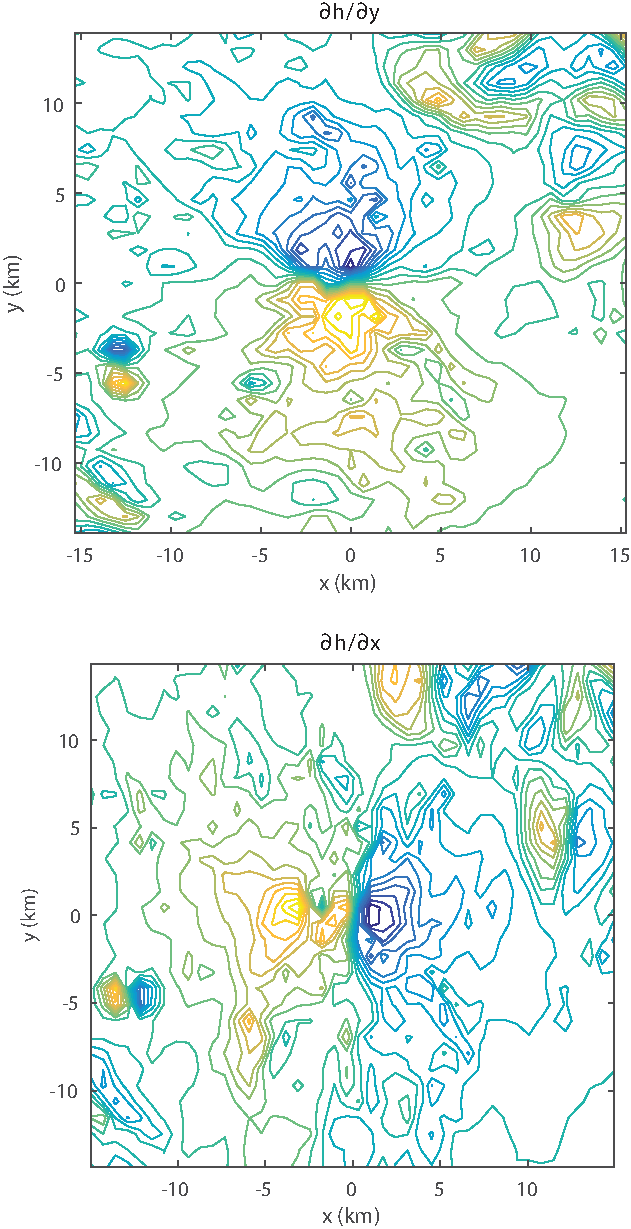
\includegraphics[width=0.75\textwidth]{activities/figures/mt_shasta_derivatives.eps}
%     \caption{Elevation derivatives of Mount Shasta region in the (top) north
%     direction and (bottom) east direction.}
%     \label{fig:ms_dxdy}
% \end{figure}

From the result above, we learn that the slope is different depending upon the direction you walk (N-S) versus (E-W) which confounds the direction of the maximum slope.  You may also note that if we had walked in the opposite (negative) directions, we would have changed the sign of our slopes.  Do not fear, there is a simple mathematical solution to determine both the maximum slope and its direction.

If we assume that from each point that we walked in either the +x or +y direction we can describe the local surface as a plane, the directions we walked were purposfully perpendicular to each other.  It turns out that these two directions can be used to define that plane and both the angle and magnitude of the maximum slope (magnitude) along it (Figure~\ref{fig:resultant}).  To determine the maximum slope along each individual little plane, we use the Pythagorean theorem, which you may remember from high school,
\begin{equation}
    \norm{s} = (s_x^2 + s_y^2)^{1/2}.
\end{equation}
Note that because we square each slope component before adding them, we have ensured that our resultant magniude of the slope is positive.  To determine the direction of the maximum slope, we can use trigonometry to determine the angle with respect to the x-axis as
\begin{equation}
    \tan \theta = \frac{s_y}{s_x}.
\end{equation}
Note that to find the appropriate angle we will have to keep track of the signs of $s_x$ and $s_y$ to ensure that $\theta$ lies in the appropriate quadrant.

\section{Marble Canyon Example}
\begin{figure}[h]
    \centering
    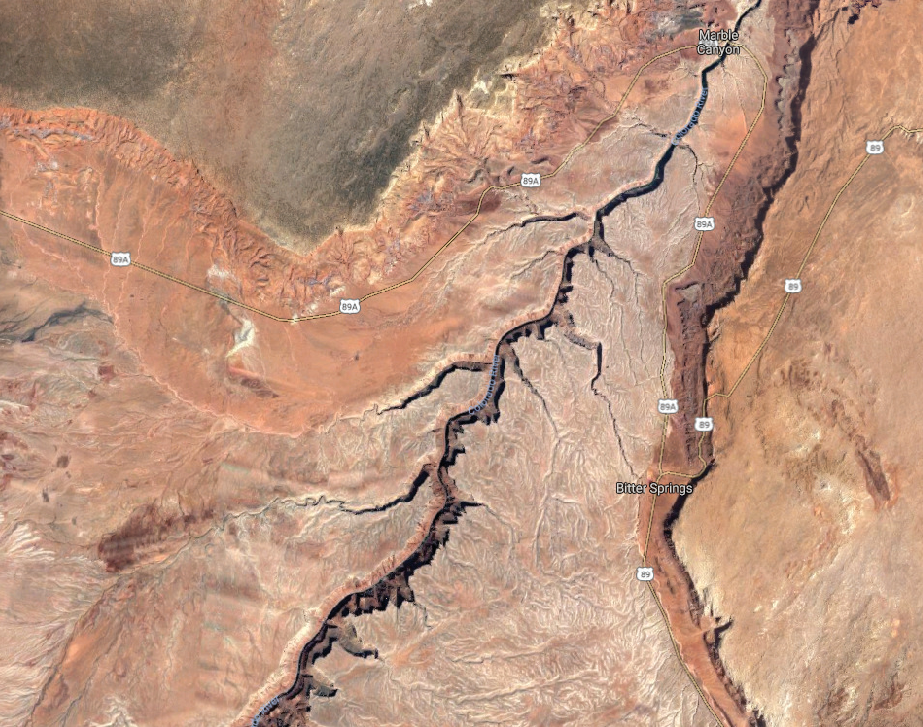
\includegraphics[width=0.75\textwidth]{activities/figures/marble_canyon.eps}
    \caption{Marble Canyon, Arizona (image from Google Earth).}
    \label{fig:mc}
\end{figure}
Let's look at another topographic example at Marble Canyon in Arizona.  Marble Canyon sits before the entrance of the Grand Canyon.  The area surrounding the canyon has relatively flat topography except for some steep-sided cliffs, one east of the canyon that runs approximately north to south and a second, north of the canyon which varies in azimuth.  The canyon itself runs northeast to southwest though the center of the image, carved by the Colorado River.

In this exercise, we will take the previous example one step further by determining the slope along each individual axis and then combine them as we might in the mathematical sense and then combine the results to obtain determine a magnitude and direction.  Again, we'll do this graphically rather than mathematically to gain further insight into how the mathematics works.  Note there is a substantial region where the topography is relatively flat (i.e., the slope is negligible).  You don't need to put any arrows in these positions so focus on regions where elevation changes.
\FloatBarrier

\begin{questions}[resume]
    \question{Marble Canyon}
    \begin{figure}[htb]
        \centering
        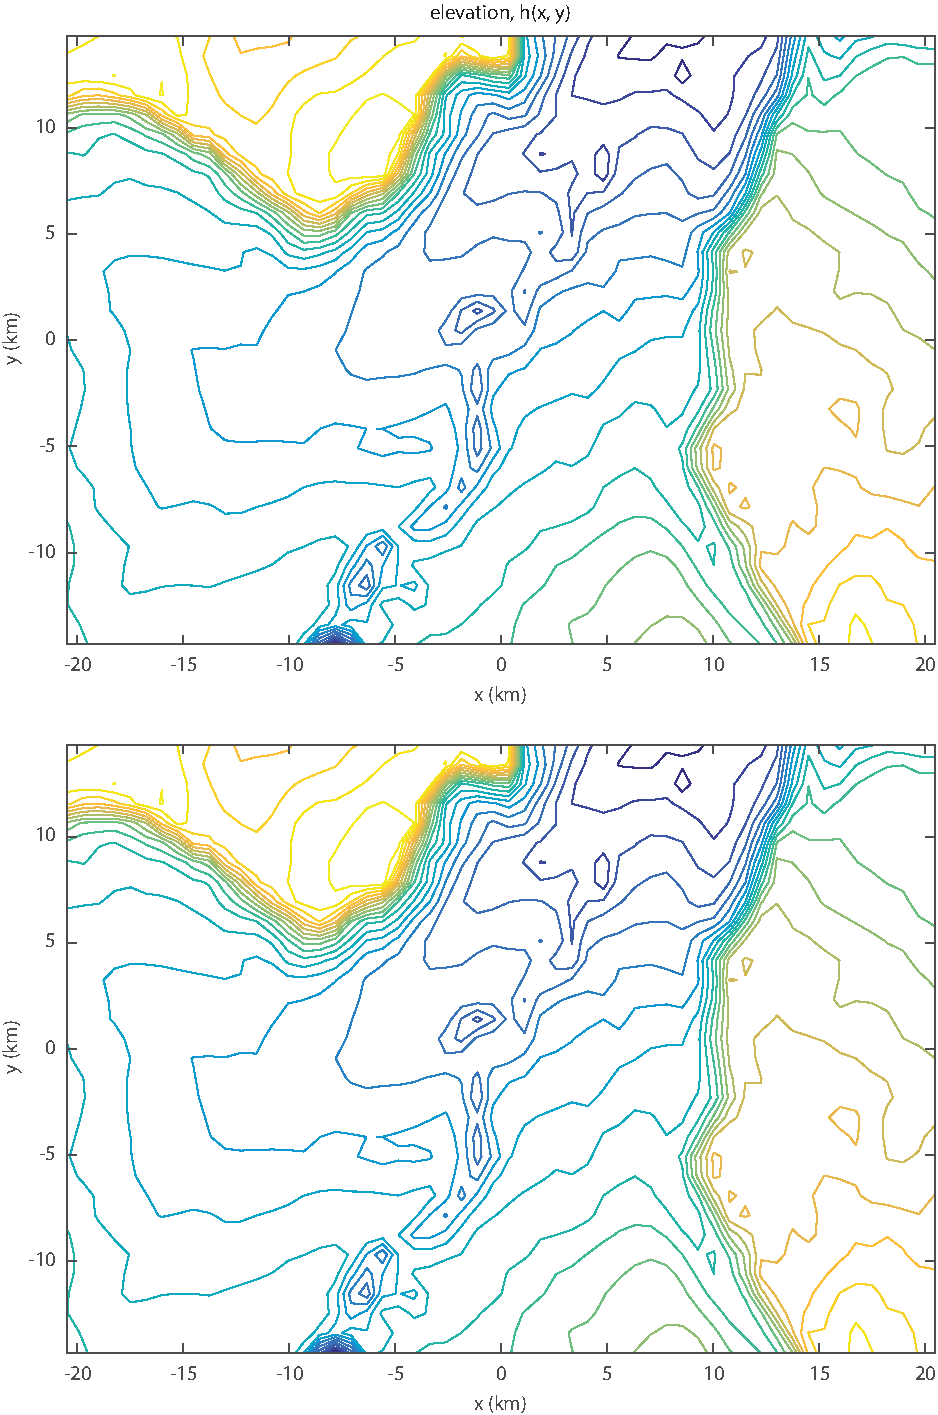
\includegraphics[width=0.6\textwidth]{activities/figures/marble_canyon_elevation.eps}
        \caption{Topographic map of Marble Canyon.}
        \label{fig:mc_elev}
    \end{figure}

    \begin{parts}
        \part In Figure~\ref{fig:mc_elev} are two of the same topographic map of Marble Canyon.  On the top map, make a series of arrows parallel to the x-axis with length represpresenting the slope in the x-direction.  Again, arrow should point up slope.  Now on the same topographic map, make a series of arrows parallel to the y-axis with length representing the slope in the y-direction.
        
        Once you have both sets of arrows, create a new set of arrows on the bottom topograpic map that represent a combination of the two.  The resultant vector is simply a graphical application of the Pythagorean equation.  What you will have done is the same thing that the math is doing.  So when we are working with abstract fields that cannot be seen or felt by us, remember, the concept is shown here is the same.

        \part How do the individual derivative components behave with respect to the ridge running north east of the canyon?
        \answerbox[3cm]

        \part For the northern ridge, why does the y-component have only positive slopes whereas the x-component is positive in some places and negative in others?
        \answerbox[3cm]

        \part Can you find examples of either of the above situations occuring in the canyon itself?
        \answerbox[2cm]
    \end{parts}
\end{questions}

% \begin{figure}[htb]
%     \centering
%     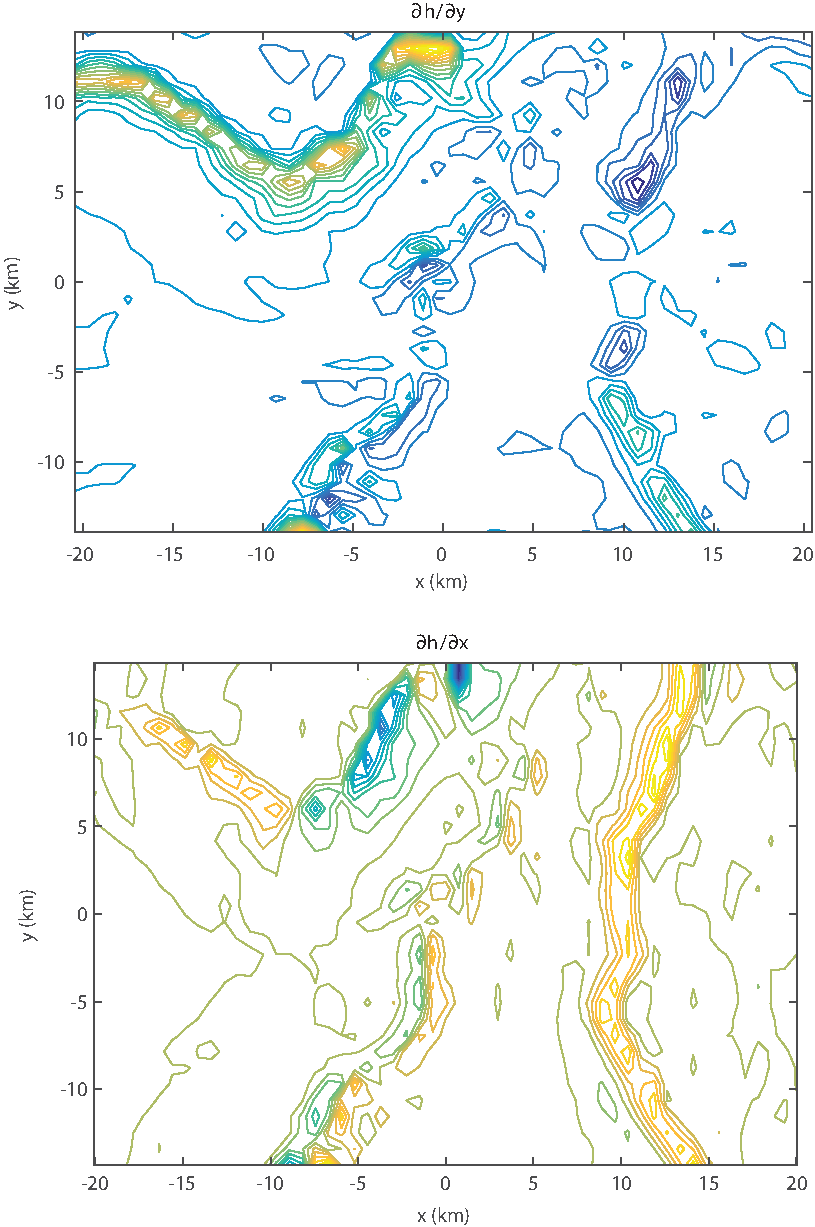
\includegraphics[width=0.75\textwidth]{activities/figures/marble_canyon_derivatives.eps}
%     \caption{Elevation derivatives of Marble Canyon region in the (top) north direction and (bottom) east direction.}
%     \label{fig:ms_dxdy}
% \end{figure}

% \begin{figure}[htb]
%     \centering
%     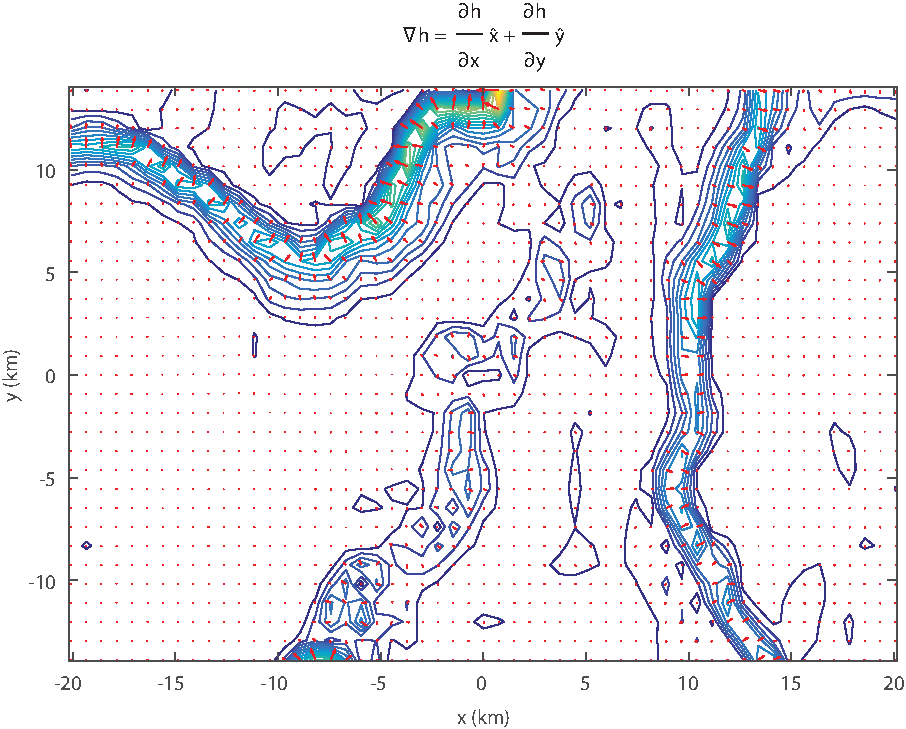
\includegraphics[width=0.75\textwidth]{activities/figures/marble_canyon_gradient.eps}
%     \caption{Gradient magnitudes (contours) and directions (arrows) of Marble Canyon.}
%     \label{fig:ms_dxdy}
% \end{figure}

\end{activity}